%# -*- coding:utf-8 -*-
\subsection[模型数据优化]{面向交互仿真的血管系统模型数据优化}

\begin{frame}
\begin{itemize}
  \item \textbf{血管表面模型优化流程}:
\end{itemize}
\begin{figure}[t]
\centering
%# -*- coding:utf-8 -*-
\begin{tikzpicture}[scale=.3]

\draw [black,thick,rounded corners] (-3,0) rectangle (3,2);            % binary threshold
\draw [black,thick,rounded corners] (-3,3) rectangle (3,5);  % GAC

\draw [black,thick,rounded corners] (-8,7) rectangle (-2,9); % fast marching
\draw [black,thick,rounded corners] (-8,13) rectangle (-2,15); % thresholding
\draw [black,thin,dashed] (-8.5,6.5) rectangle (-1.5,15.5);
\node [above right] at (-8.5,15.5) {\tiny \fs \bf 初始水平集};

\draw [black,thick,rounded corners] (2,7) rectangle (8,9);   % sigmoid
\draw [black,thick,rounded corners] (2,10) rectangle (8,12); % gradient
\draw [black,thick,rounded corners] (2,13) rectangle (8,15); % curvature anisotropic diffusion
\draw [black,thin,dashed] (1.5,6.5) rectangle (8.5,15.5);
\node [above right] at (5,15.5) {\tiny \fs \bf 特征图像};

\draw [black,thick,rounded corners] (-3,17) rectangle (3,19); % raw input

\node [above right] at (-2.1,0.25) {\tiny \fs \bf 二值阈值滤波};
\node [above right] at (-2.1,3.25) {\tiny \fs \bf 测地活动轮廓};

\node [above right] at (-6.75,7.25) {\tiny \fs \bf 快速行进};
\node [above right] at (-6.75,13.25) {\tiny \fs \bf 阈值滤波};

\node [above right] at (2.3,7.25) {\tiny \fs \bf 亮度的非线性映射};
\node [above right] at (3,10.25) {\tiny \fs \bf 梯度幅值计算};
\node [above right] at (2.3,13.25) {\tiny \fs \bf 曲率各向异性扩散};

\node [above right] at (-1.9,17.25) {\tiny \fs \bf 原始体数据};

\draw [<-,thick] (0,2) -- (0,3);

\draw [<-,thick] (0,5) -- (0,6);
\draw [thick] (-5,6) -- (5,6);
\draw [thick] (-5,6) -- (-5,7);
\draw [thick] (5,6) -- (5,7);

\draw [<-,thick] (-5,9) -- (-5,13);
\draw [<-,thick] (5,9) -- (5,10);

\draw [<-,thick] (5,9) -- (5,10);
\draw [<-,thick] (5,12) -- (5,13);

\draw [<-,thick] (-5,15) -- (-5,16);
\draw [<-,thick] (5,15) -- (5,16);
\draw [thick] (-5,16) -- (5,16);
\draw [thick] (0,16) -- (0,17);

\end{tikzpicture} 
% 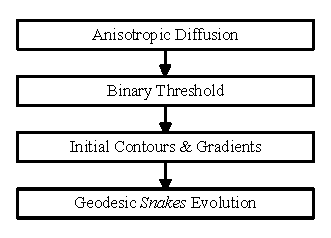
\includegraphics[width=3.2in]{Figures/gac/DataFlow.eps}
% \caption[主动脉内腔分割流程]{主动脉内腔分割流程。}
% \label{fig:aorta_data_flow}
\end{figure}
\end{frame}

\begin{frame}
\begin{itemize}
  \item \textbf{表面中顶点位置的五种情形}
  \begin{itemize}
    \item 简单情形
    \item 复杂情形
    \item 边缘情形
    \item 边缘内部情形
    \item 拐角情形
  \end{itemize}
\end{itemize}
\begin{figure}
\begin{minipage}[t]{0.8\linewidth}
\centering
% top
\subfigure[]{
\input{../../FigureSrc/postprocessing/mesh/GeneralSimple}
\quad
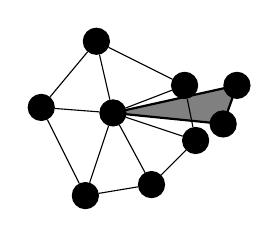
\begin{tikzpicture}[scale=.7,every node/.style={draw,shape=circle,fill=black,minimum size=1pt}]
\draw [fill=gray,thick] (0.5,1.5) -- (2.5,1.3) -- (2.75,2) -- (0.5,1.5);
% vertices
\path (0.5,1.5) node (p0) {}
(0,0) node (p1) {}
(1.2,0.2) node (p2) {}
(2,1) node (p3) {}
(1.8,2) node (p4) {}
(0.2,2.8) node (p5) {}
(-0.8,1.6) node (p6) {}
(2.5,1.3) node (p7) {}
(2.75,2) node (p8) {};
% edges
\draw (p0) -- (p1)
(p0) -- (p2)
(p0) -- (p3)
(p0) -- (p4)
(p0) -- (p5)
(p0) -- (p6)
(p1) -- (p2)
(p2) -- (p3)
(p3) -- (p4)
(p4) -- (p5)
(p5) -- (p6)
(p6) -- (p1);
\end{tikzpicture}
\quad
\input{../../FigureSrc/postprocessing/mesh/Boundary}
}
% bottom
\subfigure[]{
\input{../../FigureSrc/postprocessing/mesh/InteriorEdge}
\quad
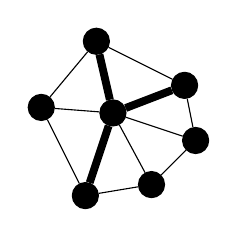
\begin{tikzpicture}[scale=.7,every node/.style={draw,shape=circle,fill=black,minimum size=1pt}]
% vertices
\path (0.5,1.5) node (p0) {}
(0,0) node (p1) {}
(1.2,0.2) node (p2) {}
(2,1) node (p3) {}
(1.8,2) node (p4) {}
(0.2,2.8) node (p5) {}
(-0.8,1.6) node (p6) {};
% edges
\draw (p0) -- (p1)
(p0) -- (p2)
(p0) -- (p3)
(p0) -- (p4)
(p0) -- (p5)
(p0) -- (p6)
(p1) -- (p2)
(p2) -- (p3)
(p3) -- (p4)
(p4) -- (p5)
(p5) -- (p6)
(p6) -- (p1);
\draw [line width=.1cm] (p1) -- (p0) -- (p4);
\draw [line width=.1cm] (p0) -- (p5);
\end{tikzpicture}
}	
\end{minipage}
\end{figure}
\end{frame}

\begin{frame}
\begin{itemize}
  \item \textbf{削减顶点引起的多边形减少}
  \begin{itemize}
    \item 简单情形:削减前的多边形数量:$6$,削减后的多边形数量:$4$
    \item 边缘情形:削减前的多边形数量:$5$,削减后的多边形数量:$4$
  \end{itemize}
\end{itemize}
\begin{figure}
\begin{minipage}[t]{0.8\linewidth}
\centering
% top
\subfigure[简单情形]{
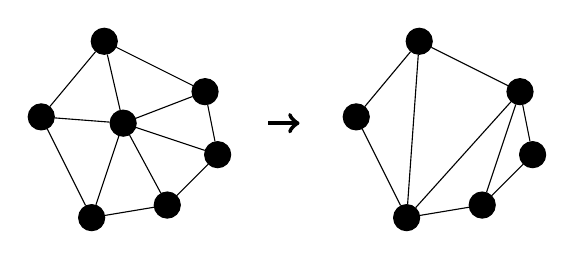
\begin{tikzpicture}[scale=.8,every node/.style={draw,shape=circle,fill=black,minimum size=3pt}]
% vertices
\path (0.5,1.5) node (p0) {}
(0,0) node (p1) {}
(1.2,0.2) node (p2) {}
(2,1) node (p3) {}
(1.8,2) node (p4) {}
(0.2,2.8) node (p5) {}
(-0.8,1.6) node (p6) {};
\path %(5.5,1.5) node (p7) {}
(5,0) node (p8) {}
(6.2,0.2) node (p9) {}
(7,1) node (p10) {}
(6.8,2) node (p11) {}
(5.2,2.8) node (p12) {}
(4.2,1.6) node (p13) {};
% edges
\draw (p0) -- (p1)
(p0) -- (p2)
(p0) -- (p3)
(p0) -- (p4)
(p0) -- (p5)
(p0) -- (p6)
(p1) -- (p2)
(p2) -- (p3)
(p3) -- (p4)
(p4) -- (p5)
(p5) -- (p6)
(p6) -- (p1);
\draw (p8) -- (p9)
(p9) -- (p10)
(p10) -- (p11)
(p11) -- (p12)
(p12) -- (p13)
(p13) -- (p8)
(p8) -- (p12)
(p8) -- (p11)
(p9) -- (p11);
% draw arrow
\draw [->,ultra thick] (2.8,1.5) -- (3.3,1.5);
\end{tikzpicture}
}
% bottom
\subfigure[边缘情形]{
\input{../../FigureSrc/postprocessing/mesh/BoundaryReduction}
}	
\end{minipage}
\end{figure}
\end{frame}

\begin{frame}
\begin{itemize}
  \item \textbf{表面模型的VOI提取及连接性检验}:
\end{itemize}
\begin{figure}[t]
\centering
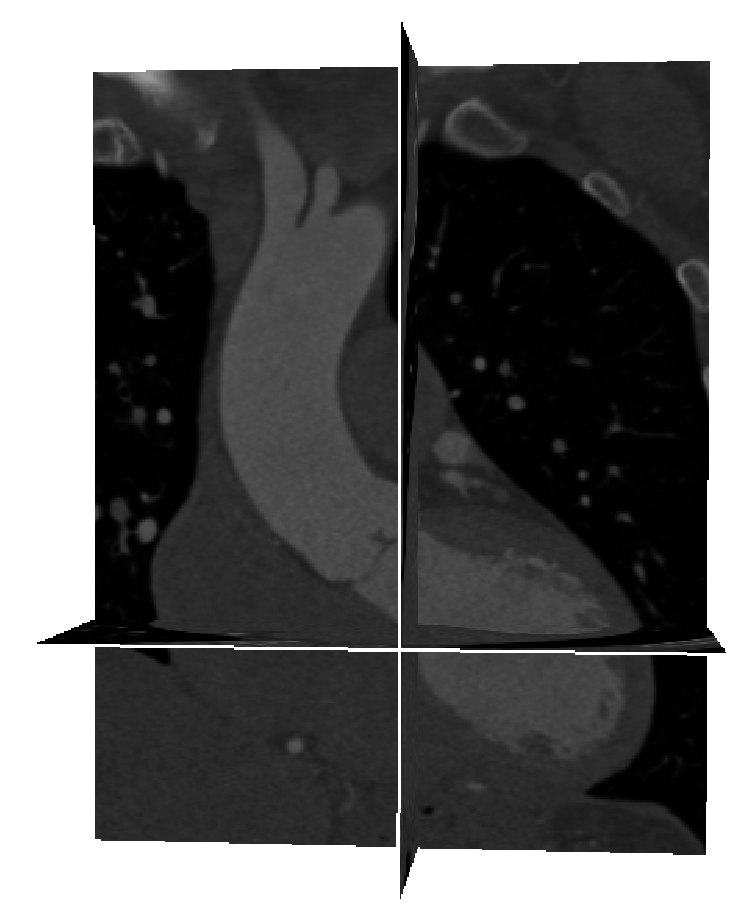
\includegraphics[height=2.0in]{../../Figures/postprocessing/mesh/original.eps}
\qquad
\raisebox{20mm}{
\centering
\renewcommand{\arraystretch}{0.5}
\begin{tabular*}{40mm}{lc}
\toprule
~                & \small{多边形数量} \\
\midrule
\small{检验前}   & \small{$74,307$}  \\
\small{检验后}   & \small{$74,307$}  \\
\bottomrule
\end{tabular*}
}
\end{figure}
% }
% \caption[表面模型的VOI提取及连接性检验]{表面模型的VOI提取及连接性检验。}
% \label{fig:mesh_connectivity}
\end{frame}

\begin{frame}
\begin{itemize}
  \item \textbf{设置不同参数获得的平滑结果(优化)}:
\end{itemize}
\begin{figure}[t]
\renewcommand{\arraystretch}{0.5}
% \caption[为平滑算法设置不同的参数所获得的结果]{为平滑算法设置不同的参数所获得的结果($N$:迭代次数;$\delta$:带宽)}
% \label{tbl:mesh_smooth}
\centering
\begin{tabular}{|l|c|c|c|}
\hline
\bigstrut ~                                   & \raisebox{-1mm}{$N = 30$}                                     & \raisebox{-1mm}{$N = 60$}                                     & \raisebox{-1mm}{$N = 100$}                                     \\
\hline
\bigstrut[t] \raisebox{0mm}{$\delta = 0.1$}  & \Includegraphics[height=1.0in]{../../Figures/postprocessing/mesh/smooth_30_1.eps}  & \Includegraphics[height=1.0in]{../../Figures/postprocessing/mesh/smooth_60_1.eps}  & \Includegraphics[height=1.0in]{../../Figures/postprocessing/mesh/smooth_100_1.eps}  \\
\hline
\bigstrut[b] \raisebox{0mm}{$\delta = 0.01$} & \Includegraphics[height=1.0in]{../../Figures/postprocessing/mesh/smooth_30_01.eps} & \Includegraphics[height=1.0in]{../../Figures/postprocessing/mesh/smooth_60_01.eps} & \Includegraphics[height=1.0in]{../../Figures/postprocessing/mesh/smooth_100_01.eps} \\
\hline
\end{tabular}
% \caption[设置不同参数获得的平滑结果(优化)]{设置不同参数获得的平滑结果。($N$:迭代次数;$\delta$:带宽)}
% \label{fig:mesh_smooth}
\end{figure}
\end{frame}

\begin{frame}
\begin{itemize}
  \item \textbf{设置不同参数获得的精简}:
\end{itemize}
\begin{figure}[t]
\begin{table}[t]
\renewcommand{\arraystretch}{0.5}
% \caption[为削减算法设置不同参数所获得的结果]{为平滑算法设置不同的参数所获得的结果($N$:迭代次数;$\delta$:带宽)}
% \label{tbl:mesh_decimate}
\centering
\begin{tabular}{|l|c|c|c|}
\hline
\bigstrut ~                                    & \raisebox{-1mm}{$10\%$}                                                                 & \raisebox{-1mm}{$90\%$}                                                               & \raisebox{-1mm}{$99\%$}                                     \\
\hline
\bigstrut[t] \raisebox{0mm}{\small{表面模型}} & \Includegraphics[height=1.0in]{../../Figures/postprocessing/mesh/smooth_100_01_d10.eps}     & \Includegraphics[height=1.0in]{../../Figures/postprocessing/mesh/smooth_100_01_d90.eps}   & \Includegraphics[height=1.0in]{../../Figures/postprocessing/mesh/smooth_100_01_d99.eps}   \\
\hline
\bigstrut[b] \raisebox{0mm}{\small{线框模型}} & \Includegraphics[height=1.0in]{../../Figures/postprocessing/mesh/smooth_100_01_d10_w.eps}   & \Includegraphics[height=1.0in]{../../Figures/postprocessing/mesh/smooth_100_01_d90_w.eps} & \Includegraphics[height=1.0in]{../../Figures/postprocessing/mesh/smooth_100_01_d99_w.eps} \\
\hline
\end{tabular}
% \caption[设置不同参数获得的精简]{设置不同参数获得的精简:上排展示了削减率分别为$10\%$,$90\%$,$99\%$时的结果;下排展示了上排相应削减结果所对应的线框表示。}
% \label{fig:mesh_decimate}
\end{table}
\end{figure}
\end{frame}

\begin{frame}
\begin{itemize}
  \item \textbf{削减率与削减后的多边形数量}:
\end{itemize}
\begin{table}[h]
\renewcommand{\arraystretch}{0.5}
% \caption[削减率与削减后的多边形数量]{削减率与削减后的多边形数量}
% \label{tbl:mesh_decimate}
\centering
\begin{tabular*}{100mm}{c r r r r r}
\toprule
% \bfseries      & \bfseries Quantity of polygonal surfaces \\
\hspace{2mm} \small{削减率 ($\%$)}  &     \small{$10$} &     \small{$50$} &     \small{$75$} &    \small{$90$} &  \small{$99$} \\
\midrule
\hspace{2mm} \small{多边形数量}     & \small{$66,875$} & \small{$37,153$} & \small{$18,576$} & \small{$7,430$} & \small{$743$} \\
\bottomrule
\end{tabular*}
\end{table}
\end{frame}

\begin{frame}
\begin{itemize}
  \item \textbf{精简率与fps——情形I}:
\end{itemize}
\begin{table}[t]
\renewcommand{\arraystretch}{0.5}
% \caption[精简率与fps——情形I]{精简率与fps——情形I}
% \label{tbl:mesh_FPS1}
\centering
\begin{tabular*}{100mm}{c r r r r r}
\toprule
\hspace{5mm} \small{精简率($\%$)}           & \small{$10$} & \small{$50$} & \small{$75$} & \small{$90$} & \small{$99$} \\
\midrule
\hspace{5mm} \small{仿真初始fps}              & \small{$30$} & \small{$35$} & \small{$38$} & \small{$41$} & \small{$42$} \\
\midrule
\hspace{5mm} \small{仿真平均fps}              &  \small{$6$} & \small{$10$} & \small{$15$} & \small{$18$} & \small{$30$} \\
\midrule
\hspace{5mm} \small{是否完成仿真?(是/否)}  &  \small{否}  &  \small{否}  & \small{是}   & \small{是}   & \small{是}   \\
\bottomrule
\end{tabular*}
\end{table}
\end{frame}

\begin{frame}
\begin{itemize}
  \item \textbf{精简率与fps——情形II}:
\end{itemize}
\begin{table}[t]
\renewcommand{\arraystretch}{0.5}
% \caption[精简率与fps——情形II]{精简率与fps——情形II}
% \label{tbl:mesh_FPS2}
\centering
\begin{tabular*}{80mm}{c r r r r r}
\toprule
\hspace{5mm} \small{精简率($\%$)}           & \small{$90$} & \small{$95$} & \small{$99$} \\
\midrule
\hspace{5mm} \small{仿真初始fps}              & \small{$20$} & \small{$32$} & \small{$31$} \\
\midrule
\hspace{5mm} \small{仿真平均fps}              &  \small{$4$} &  \small{$6$} & \small{$11$} \\
\midrule
\hspace{5mm} \small{是否完成仿真?(是/否)}  &  \small{否}  &  \small{否}  & \small{是}   \\
\bottomrule
\end{tabular*}
\end{table}
\end{frame}

\begin{frame}

\end{frame} 